\documentclass[10pt,a4paper]{report}
\usepackage[utf8]{inputenc}
\usepackage[T1]{fontenc}
\usepackage{amsmath}
\usepackage{amsfonts}
\usepackage{amssymb}
\usepackage{graphicx}
\usepackage{hyperref}
\usepackage{xcolor}
\begin{document}
\definecolor{ao}{rgb}{0.0, 0.0, 1.0}
\begin{center}
	\begin{minipage}{0.4\textwidth}
		\begin{flushleft}
    			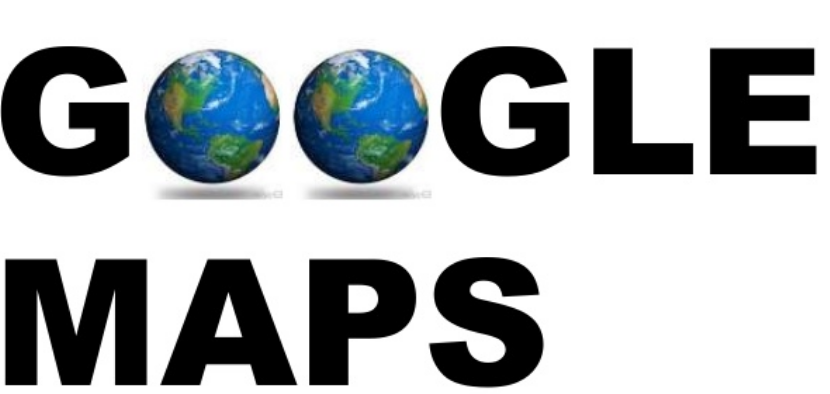
\includegraphics[scale=0.2]{1.png}
		\end{flushleft}
	\end{minipage}
	\begin{minipage}{0.4\textwidth}
		\begin{flushright}
			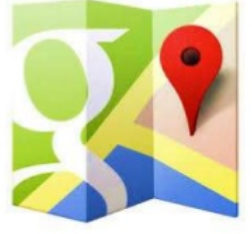
\includegraphics[scale=0.1]{2.png}
		\end{flushright}
	\end{minipage}
\end{center} 


\textbf{History and Presentation of Google Maps :}
\begin{itemize}
\item Google Maps is a platform, developed by the American giant Google, which generates a world map. It is therefore a Web application covering a directory tool and global map data.
\item Launched in 2004 in the United States and Canada, and in 2005 in Great Britain (known as Google Local), Google Maps was launched on Thursday, April 27, 2006, simultaneously in France, Germany, Spain and Italy. And since then, Google through these tools and its community, is successfully mapping the world.
\item The Google Maps database can be queried as a traditional intelligence service to locate a location, a business, calculate or route, or vice versa to visually search for previously indexed locations on a map.
\item This service allows you to zoom in to a street scale from one country. Still shots showing the details of certain streets are also available. You can search for a place in the world or draw routes between two places.
\end{itemize}
\textbf{How to use Google Maps ?}\\
You can use Google Maps on your computer, phone, or tablet to search, explore, and find where you are. 
\begin{itemize}
\item On your computer, open Google Maps here: \textcolor{ao}{\href{http://maps.google.ci/}{http://maps.google.ci/}}.
\item On your phone or tablet, use the Google Maps app to download it to play store (for Andriod phones) or apple store (for Apple phones).
\end{itemize}
\textbf{Started with the Google Maps app : }\\
Are you new to the Google Maps app?\\
This step-by-step guide teaches you how get set up and learn the basics.
When you finish the guide, you’ll know how to find info about a place and how to get there. And you’ll save time because the Maps app will know your home and work addresses.
\begin{itemize}
\item Sign in to an account or change account :\\
When you sign in to Google Maps, you can:
\begin{itemize}
\item quickly find your favorite places.
\item obtain better research results.
\item register the address of your home and the address of your place of work.
\end{itemize}

\item  Save your home and work :\\
Type less by saving your home and work addresses. And then shorten your commute by getting the fastest route :
\begin{itemize}
\item Open the Google Maps app.
\item Tap Menu $\equiv$ > Your Places and > Enter home or work address.
\end{itemize}
\item Get info about a place :\\
Find a place on the map to get directions. Or get info like business hours, menus, and see Street View imagery.
\begin{itemize}
\item Open the Google Maps app.
\item Search for a place or tap it on the map.
\item Swipe up on the info sheet.
\end{itemize}
\item Start navigation :
\begin{itemize}
\item Open the Google Maps app.
\item Get directions to a location.
\item To hear voice-guided navigation, tap Sound.
\item To exit navigation, in the lower left, tap Close.
\end{itemize}
\end{itemize}
\textbf{Google Maps gives us three types of views :}
\begin{itemize}
\item A classic plan view, with street names, neighborhood, cities.
\begin{center}
	
\includegraphics[scale=0.3]{3.png}
\end{center}
\item A satellite image view, which today covers the entire world.
\begin{center}
	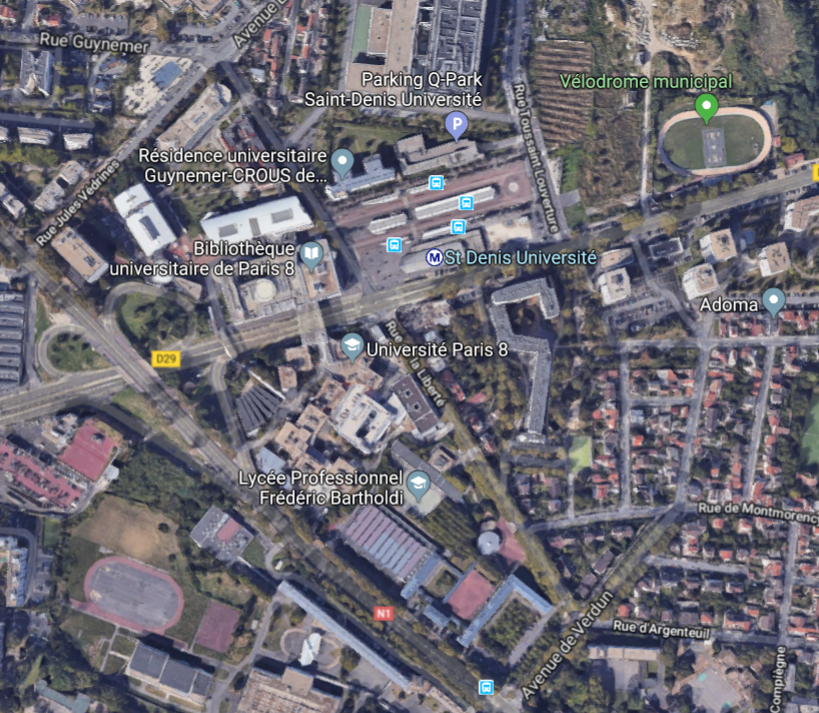
\includegraphics[scale=0.2]{4.png}
\end{center}
\item A 3D earth view.
\begin{center}
	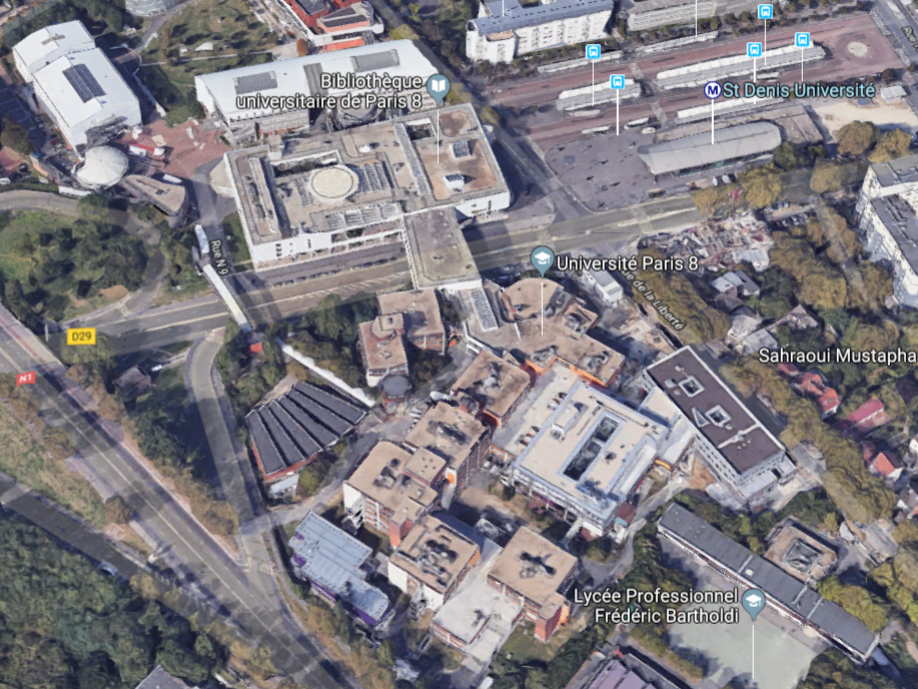
\includegraphics[scale=0.2]{5.png}
\end{center}
\end{itemize}
\textbf{The different service :}
\begin{center}
	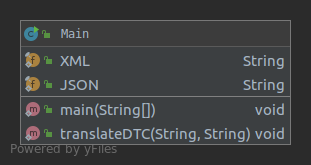
\includegraphics[scale=0.3]{6.png}
\end{center}
My favor option is your timeline this tools allows us to follow our route already done with all possible details.
\begin{center}
	\begin{minipage}{0.4\textwidth}
		\begin{flushleft}
    			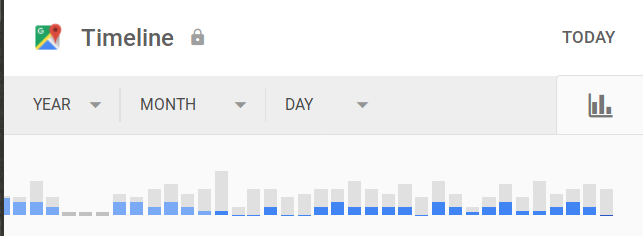
\includegraphics[scale=0.3]{7.png}
		\end{flushleft}
	\end{minipage}
	\begin{minipage}{0.4\textwidth}
		\begin{flushright}
			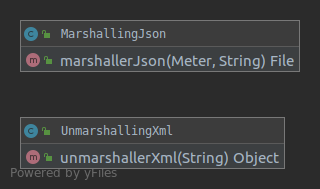
\includegraphics[scale=0.2]{8.png}
		\end{flushright}
	\end{minipage}
\end{center} 
\end{document}